\documentclass{article}
\usepackage{graphicx}
\usepackage[utf8]{inputenc}
\usepackage{booktabs}
\usepackage{array}
\usepackage{longtable}
\usepackage{amsmath}
\usepackage[letterpaper, margin=1in]{geometry}

\usepackage[
backend=biber,
style=alphabetic,
sorting=ynt
]{biblatex}
 
\addbibresource{refs.bib}

\newcolumntype{L}[1]{>{\raggedright\let\newline\\\arraybackslash\hspace{0pt}}m{#1}}
\newcolumntype{C}[1]{>{\centering\let\newline\\\arraybackslash\hspace{0pt}}m{#1}}
\newcolumntype{R}[1]{>{\raggedleft\let\newline\\\arraybackslash\hspace{0pt}}m{#1}}


\title{code-smells}
\author{ }
\date{July 2015}

\begin{document}

\maketitle

\section{Code Smell list}

\begin{table}[ht]
\centering
\begin{tabular}{l|l|c|c|c|c}
 Code Smells~\cite{Fowler99} & Marinescu~\cite{Lanza2006} & SonarQube\textsuperscript{\textdagger} & Rank~\cite{Yamashita2013} & \cite{Atwood06}\textsuperscript{\textdaggerdbl} & Keymind Rank\textsuperscript{\textexclamdown}\\
 \toprule
  Alt. Classes with Diff. Interfaces & & & & + & \\
  Combinatorial Explosion~\cite{Kerievsky2004} & & & & + & \\
  Comments & & & 11 & + & VL\\
  Conditional Complexity~\cite{Kerievsky2004} & & & 14 & + & ?\\
  Data Class & Data Class & & & + &\\
  Data Clumps &  &  & & + &\\
  Divergent Change & & & & + & \\
  Duplicated Code & Significant Duplication\textsuperscript{*} & + & 1 & + & VH\\
  Feature Envy & Feature Envy & & 8 & + &\\
  
  Inappropriate Intimacy & & - & & + & L\\
  Indecent Exposure~\cite{Kerievsky2004} & & & & + & ?\\
  Incomplete Library Class & & & & + &\\
  Large Class & God Class/Brain Class & ++ & 4 & + & VH\\
  Lazy Class/Freeloader & & - & 7 & + &\\
  Long Method & Brain Method & ++ & 2 & + & VH\\
  Long Parameter List &  & + & 9 & + & L \\
  
  Message Chains & & & & + & H\\
  Middle Man & &  & & + &\\
  Oddball Solution~\cite{Kerievsky2004} & & & & + & \\
  Parallel Inheritance Hierarchies & & & & + &\\
  Primitive Obsession &  & & & + &\\
  
  Refused Bequest & Refused Parent Bequest & - & & + & \\ 
  Shotgun Surgery & Shotgun Surgery & & & + & \\
  Solution Sprawl~\cite{Kerievsky2004} & & & & + &\\
  Speculative Generality & & & & + & L\\
  Switch Statements &  & - & & & L\\
  Temporary Field & & - & & + & ?\\
  \multicolumn{5}{l}{} \\
  \multicolumn{5}{l}{\textsuperscript{\textdagger} + Exact rule, - Possibly related rule} \\
    \multicolumn{5}{l}{\textsuperscript{\textdaggerdbl} + is included in list} \\
    \multicolumn{5}{l}{\textsuperscript{\textexclamdown} VH: Very High, H: High, L: Low, VL: Very Low, ?: Still investigating} \\
   \multicolumn{5}{l}{\textsuperscript{*} Computation is based on more than simple metrics.} \\

\end{tabular}
\caption{List of code smells from~\cite{Fowler99} and~\cite{Kerievsky2004}}
\label{tab:smells}
\end{table}

\section{Related Work}

\begin{figure}
\centering
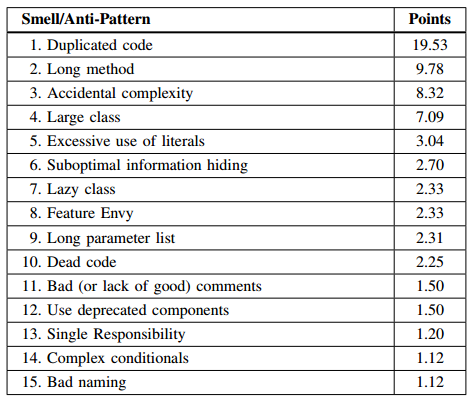
\includegraphics[scale=0.75]{Yama_smell_ranking}
\caption{RANKING OF MOST POPULAR CODE SMELLS/ANTI-PATTERNS from \cite{Yamashita2013}}
\label{fig:yama_smell_ranking}
\end{figure}

Summary:
\begin{itemize}
\item Contradictory empirical evidence that code smells is associated with faults or maintenance effort.
\item Subjective assessment of code smells does not agree with automated detection of smells.
\item Developers don't agree on what is smelly. Developers also don't concur on the importance or impact of smells.
\end{itemize}


Fowler99 - Fowler and Beck introduce the concept of ''code smells' and provide a list of smells with qualitative description.\cite{Fowler99}

Mantyla2003 - Created taxonomy in Table~\ref{tab:smells}. \cite{Mantyla2003}

Marinescu2004 - Original paper on automated code smell detection. Discusses accuracy. Applied to two large (700K and 2000k) telecommunication software systems.\cite{Marinescu2004}

Mantyla2004 - Human subjective evaluation v. metrics-based detection of three code smells (Large Class, Long Parameter List, and Duplicate code) in a Finnish software company. Tools used: \url{http://sourceforge.net/projects/same} and \url{http://www.sdmetrics.com/}. We studied the subjective smell evaluations of developers and noticed that demographic data (knowledge, role, workexperience) seemed to explain some of the variances in smell evaluations. Also, when we studied the uniformity of the smell evaluations, we saw how the subjective smell evaluations are affected by conflicting perceptions of different developers. We also applied source code metrics for three smells and compared the results to the subjective smell evaluations. It appears that developers’ evaluations of the smells do not correlate with the used source code metrics.\cite{Mantyla2004}

Mantyla2006 - Finnish software company software modules. We found that the use of smells for code evaluation purposes can be difficult due to conflicting perceptions of different evaluators. However, the demographics of the evaluators partly explain the variation. Second, we applied selected source code metrics for identifying four smells (Large Class, Long Method, Long Parameter List, Duplicate Code) and compared these results to the subjective evaluations. The metrics based on automatic program analysis and the human-based smell evaluations did not fully correlate. Based upon our results, we suggest that organizations should make decisions regarding software evolvability improvement based on a combination of subjective evaluations and code metrics.\cite{Mantyla2006}

Lanza2006 - Extension of Marinescu's dissertation~\cite{Marinescu02}. Contains metric definitions and detection strategy definitions for some code smells. Also contains threshold values (e.g. VERY HIGH = ?, FEW = ?) for Java and C++ systems based pn 45 java and 37C++ systems.

Olbrich2010 - It is claimed that classes that are involved in certain code smells are liable to be changed more frequently and have more defects than other classes in the code. We investigated the extent to which this claim is true for God Classes and Brain Classes, with and without normalizing the effects with respect to the class size. We analyzed historical data from 7 to 10 years of the development of three open-source software systems. The results show that God and Brain Classes were changed more frequently and contained more defects than other kinds of class. However, when we normalized the measured effects with respect to size, then God and Brain Classes were less subject to change and had fewer defects than other classes.\cite{Olbrich2010} 

Olbrich2009 - GodClass and Shotgun Surgery smells studied in two open source systems. With regard to change behavior, in this study the classes infected with code smells have a higher change frequency; such classes seem to need more maintenance than non-infected classes; furthermore God Classes feature bigger changes Thus, the probability is higher that maintenance tasks take more effort since more modifications to the code (i.e., modifying, adding or deleting) is required. Initially we made the assumption that classes infected with shotgun surgery would have a lower change frequency since people would be hesitant to touch them because this implies too many changes on coupled classes and thus too much effort. The results here show that, in fact, those classes are touched much more than normal classes.\cite{Olbrich2009}

Yamashita2013 - Survey of freemarket software developers. It remains open to debate whether or not code smells should be considered meaningful conceptualizations of code quality issues from the developer’s perspective. Exploratory survey involving 85 professional software developers~\cite{Yamashita2013}. Code smells were ranked by number of survey respondents who mentioned a particular smells (Figure~\ref{fig:yama_smell_ranking}).

Sjoberg2013 - Six developers were hired to perform three maintenance tasks each on four functionally equivalent Java systems originally implemented by different companies. Each developer spent three to four weeks. In total, they modified 298 Java files in the four systems. None of the 12 investigated smells was significantly associated with increased effort after we adjusted for file size and the number of changes; Refused Bequest was significantly associated with decreased effort. File size and the number of changes explained almost all of the modeled variation in effort. Conclusion: The effects of the 12 smells on maintenance effort were limited. To reduce maintenance effort, a focus on reducing code size and the work practices that limit the number of changes may be more beneficial than refactoring code smells.\cite{Sjoberg2013}
\begin{itemize}
\item Smells detected by InCode 2.0.7 and Borland Together
\item \textbf{Data Class}
\item Data Clump
\item ''Duplicated code in conditional branches''
\item \textbf{Feature Envy}
\item \textbf{God Class}
\item \textbf{God Method}
\item Interface Segregation Principle Violation
\item Misplaced Class
\item \textbf{Refused Bequest}
\item \textbf{Shotgun Surgery}
\end{itemize}




\clearpage


\section{Marinescu Metrics}

\begin{table}[!h]
\centering
\begin{tabular}{L{4cm}|L{12cm}}
 AMW -- Average Method Weight & The average static complexity of all methods in a class.\cite{Marinescu02} McCabe's cyclomatic number~\cite{McCabe76} is used to quantify the method's complexity. \\
 \midrule
 ATFD -- Access to Foreign Data & Then number of attributes from unrelated classes that are accessed directly or by invoking accessor methods.\cite{Marinescu02} \\
 \midrule
 BOvR -- Base Class Overriding Ratio & The number of methods of the measures class that override methods from the base class, divded by the total number of methods in the class.\cite{Lanza2006} \\
 \midrule
 BUR -- Base Class Usage Ration & The numebr of inheritance-specific members used by the measured class, divided by the total number of inheritance-specific members from the base class.\cite{Lanza2006} \\
 \midrule
 CC -- Changing Classes & The number of classes in which the methods that call the measured method are defined in~\cite{Marinescu02}.\\
 \midrule
 CM -- Changing Methods & The number of disctinct methods that call the measured method \cite{Marinescu02} \\
 \midrule
 CYCLO -- McCabe's Cyclomatic Number & The number of linearly-independent paths through an operation\cite{McCabe76} \\
 \midrule
 FDP -- Foreign Data Providers & The number of classes in which the attributed accessed -- in conformity with the ATFD metric -- are defined.\cite{Lanza2006} \\
 \midrule
 LAA -- Locality of Attribute Accesses & The number of attributes from the method's deifnition class, divided by the total number of variables accessed (including attributes used via accessor methods, see ATFD), whereby the number of local attributes accessed is computed in conformity with the LAA specifications.\cite{Lanza2006} \\
 \midrule
 MAXNESTING -- Maximum Nesting Level & The maximum nesting Level of control structures within an operation\cite{Lanza2006}\\
 \midrule
 NOAM -- Number of Accessor Methods & The number of accessor (getter and setter) methods of a class\cite{Lanza2006}\\
 \midrule
 NOM -- Number of Methods & The number of methods of a class. \\
 \midrule
 NOPA -- Number of Public Attributes & the number of public attributes of a class \\
 \midrule
 NProtM -- Number of Protected Members & The number of protected methods and attributes of a class. \\
 \midrule
 TCC - Tight Class Cohesion & The relative number of method pairs of a class that access in common at least one attribute of the measured class.\cite{Bieman1995} \\
 \midrule
 WOC - Weight Of a Class & The number of ''functional'' public methods divided by the total number of public members\cite{Marinescu02}.
\end{tabular}
\caption{Marinescu metric definitions~\cite{Lanza2006}}
\label{tab:mmdefs}
\end{table}

\begin{table}[h]
\centering
\begin{tabular}{l|l}
 Value & Definition \\
 \toprule
 Lower margin & $AVG - STDEV$\\
 Average & $AVG$\\
 Higher margin & $AVG + STDEV$ \\
 Very high & $(AVG + STDEV) * 1.5$ \\
 \midrule
 NONE & 0 \\
 ONE/SHALLOW & 1 \\
 TWO, THREE/FEW/SEVERAL & 2--5 \\
 Short Memory Capacity & 7--8
\end{tabular}
\caption{Threshold terms defined in \cite{Lanza2006}}
\label{tab:thresholds}
\end{table}



\subsection{God Class}

God Class equation from~\cite{Lanza2006}:
\begin{equation}
GodClass(Class) = \begin{cases} 
                        1 & \!\begin{aligned} 
                          & {((WMC \geq \text{VERY HIGH}) \land (TCC < \text{ONE THIRD}) \land (ATFD > \text{FEW}))} 
                          \end{aligned} \\
                        0 & \text{\textit{else}} 
                  \end{cases} 
\label{eq:godclass}
\end{equation}

\subsection{Feature Envy}
Feature Envy equation from~\cite{Lanza2006}:

\begin{equation}
\text{FeatureEnvy(Method)} = 
    \begin{cases}
        1 & \!\begin{aligned}
                & (ATFD > \text{FEW}) \land (LAA < \text{ONE THIRD}) \land (FDP \leq \text{FEW}) 
            \end{aligned} \\ 
                        0 & \text{\textit{else}} 
        \end{cases} 
\label{eq:featureenvy}
\end{equation}

\subsection{Data Class}
Data Class equation from~\cite{Lanza2006}:

\begin{equation}
DataClass(Class) = \begin{cases} 
                        1 & \!\begin{aligned} 
                                & (WOC < \text{ONE THIRD})~\land \\ 
                                & ( \\
                                & \quad  ((NOPA + NOAM > \text{FEW}) \land (WMC < \text{HIGH})) \\
                                & \quad \quad \lor \\ 
                                & \quad ((NOPA + NOAM > \text{MANY}) \land (WMC < \text{VERY HIGH})) \\
                                & )
                                \end{aligned} \\
                        0 & \text{\textit{else}} \\
                    \end{cases} 
\label{eq:dataclass}
\end{equation}

\subsection{Brain Method}
Brain Method equation from~\cite{Lanza2006}:
\begin{equation}
BrainMethod(Method) = 
    \begin{cases}
        1 & \!\begin{aligned}
                & (LOC > \text{HIGH}/2) \land (CYCLO \geq \text{HIGH})~\land \\
                & (MAXNESTING \geq \text{SEVERAL}) \land (NOAV > \text{MANY}) 
            \end{aligned} \\ 
                        0 & \text{\textit{else}} 
        \end{cases} 
\label{eq:brainmethod}
\end{equation}

\subsection{Shotgun Surgery}
Shotgun Surgery equation from~\cite{Lanza2006}:
\begin{equation}
ShotgunSurgery(Method) = 
    \begin{cases}
        1 & \!\begin{aligned}
                & (CM > \text{Short Memory Cap}) \land (CC > \text{MANY})
            \end{aligned} \\ 
                        0 & \text{\textit{else}} 
        \end{cases} 
\label{eq:surgery}
\end{equation}

\subsection{Refused Parent Bequest}
\begin{equation}
DataClass(Class) = \begin{cases} 
                        1 & \!\begin{aligned} 
                                & ((NProtM > \text{FEW}) \land (BUR < \text{ONE THIRD})) \lor (BOvR < \text{ONE THIRD}) \\
                                & \land \\
                                & ((AMW > \text{AVERAGE}) \lor (WMC > \text{AVERAGE})) \land (NOM > \text{AVERAGE})
                                \end{aligned} \\
                        0 & \text{\textit{else}} \\
                    \end{cases} 
\label{eq:refusedbequest}
\end{equation}

\clearpage

\section{SonarQube ''brain overload'' rules}
\begin{longtable}{L{3cm}|L{8cm}|L{1cm}|L{1cm}}
rule & description & threshold & \cite{Atwood06} \\
\toprule
 "switch case" clauses should not have too many lines & The switch statement should be used only to clearly define some new branches in the control flow. As soon as a case clause contains too many statements this highly decreases the readability of the overall control flow statement. In such case, the content of case clause should be extracted in a dedicated method. & 5 & Sorta \\
 \midrule
"switch" statements should not have too many "case" clauses & When switch statements have a large set of case clauses, it is usually an attempt to map two sets of data. A real map structure would be more readable and maintainable, and should be used instead. & 30 & Sorta\\
\midrule
A field should not duplicate the name of its containing class & Best practice dictates that any field or member with the same name as the enclosing class be renamed to be more descriptive of the particular aspect of the class it represents or holds. & -- & No \\
\midrule
Classes should not be coupled to too many other classes (Single Responsibility Principle) & Classes which rely on many other classes tend to aggregate too many responsibilities and should be split into several smaller ones. Nested classes dependencies are not counted as dependencies of the outer class. & 20 & Sorta \\ 
\midrule
Classes should not be too complex & The Cyclomatic Complexity is measured by the number of \&\& and || operators and if, while, do, for, ?:, catch, switch, case, return and throw statements in the body of a class plus one for each constructor, method, static initializer, or instance initializer in the class. The last return statement in method, if exists, is not taken into account. & 200 & Sorta \\ 
\midrule
Control flow statements "if", "for", "while", "switch" and "try" should not be nested too deeply & Nested if, for, while, switch and try statements is a key ingredient for making what's known as "Spaghetti code". Such code is hard to read, refactor and therefore maintain. & 3 & Sorta \\
\midrule
Expressions should not be  too complex & The complexity of an expression is defined by the number of \&\&, || and condition ? ifTrue : ifFalse operators it contains. A single expression's complexity should not become too high to keep the code readable. & 3 & Sorta \\
\midrule
Fields and methods should not have conflicting names & Typically this situation indicates poor naming. Method names should be action-oriented, and thus contain a verb, which is unlikely in the case where both a method and a member have the same name. However, renaming a public method could be disruptive to callers. Therefore renaming the member is the recommended action. & -- & No \\
\midrule
Files should not have too many lines & A source file that grows too much tends to aggregate too many responsibilities and inevitably becomes harder to understand and therefore to maintain. Above a specific threshold, it is strongly advised to refactor it into smaller pieces of code which focus on well defined tasks. Those smaller files will not only be easier to understand but also probably easier to test. & 1000 & Yes \\
\midrule
Loops should not contain more than a single "break" or "continue" statement & One break and continue statement is acceptable in a loop, since it facilitates optimal coding. If there is more than one, the code should be refactored to increase readability. & 1 & No \\
\midrule
Magic numbers should not be used & A magic number is a number that comes out of nowhere, and is directly used in a statement. Magic numbers are often used, for instance to limit the number of iterations of a loops, to test the value of a property, etc. & -- & No \\
\midrule
Methods should not be too complex & The cyclomatic complexity of methods should not exceed a defined threshold. Complex code can perform poorly and will in any case be difficult to understand and therefore to maintain. & 10 & Sorta \\
\midrule
Methods should not contain too many return statements & Having too many return statements in a method increases the method's essential complexity because the flow of execution is broken each time a return statement is encountered. This makes it harder to read and understand the logic of the [method|function]. & 3 & No \\
\midrule
Methods should not have too many lines & A method that grows too large tends to aggregate too many responsibilities. Such method inevitably become harder to understand and therefore harder to maintain. Above a specific threshold, it is strongly advised to refactor into smaller methods which focus on well-defined tasks. Those smaller method will not only be easier to understand, but also probably easier to test. & 100 & Yes \\
\midrule
Methods should not have too many parameters & A long parameter list can indicate that a new structure should be created to wrap the numerous parameters or that the function is doing too many things. & 7 & Yes \\
\midrule
The ternary operator should not be used & While the ternary operator is pleasingly compact, it's use can make code more difficult to read. It should therefore be avoided in favor of the more verbose if/else structure. & -- & No \\
\caption{SonarQube ''brain overload'' rules~\cite{sonarqube15}} 
\label{tab:sonarqube}
\end{longtable}


\begin{figure}
\centering
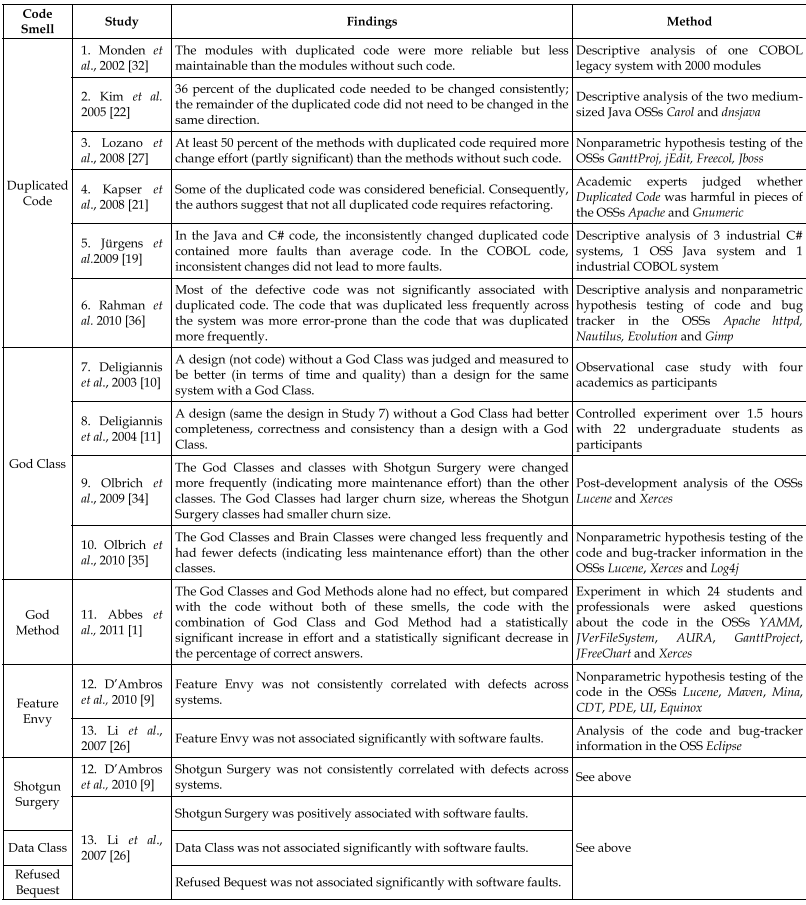
\includegraphics[width=\textwidth]{smell_studies.PNG}
\caption{Related work on Code Smells from \cite{Sjoberg2013}}
\label{fig:rw}
\end{figure}

\printbibliography
\end{document}

